\documentclass[a4paper,10pt]{report}

\usepackage{graphicx}
\usepackage{color}

\usepackage{caption}
\usepackage{subcaption}

\usepackage[portuguese]{babel}
\usepackage[utf8]{inputenc}
\usepackage[T1]{fontenc}

\usepackage{geometry}
\geometry{a4paper}
\usepackage[parfill]{parskip}

\usepackage{changepage}

\usepackage{amsmath}

\usepackage{fancyhdr}

\usepackage{nopageno}

\graphicspath{{./imagens/}}

\usepackage{url}

\usepackage{verbatim}
\usepackage{fancyvrb}

\usepackage[colorlinks=true,linkcolor=blue,citecolor=blue]{hyperref}

\usepackage{listings}
\renewcommand{\lstlistingname}{Código}
\usepackage{color}
\definecolor{grey}{rgb}{0.9,0.9,0.9}
\definecolor{greyD}{rgb}{0.5,0.5,0.5}

\lstnewenvironment{code}[1][]%
{
   \noindent
   \lstset{
	language=java,
	float=htpb,
	backgroundcolor=\color{grey},
	basicstyle=\scriptsize,
	numbers=left,
	numbersep=5pt,
	numberstyle=\tiny\color{greyD},
	breaklines=true,
	frame=single,
	#1}
}
{}

\begin{document}

\begin{titlepage}
\begin{center}

\begin{flushleft}

\includegraphics[height=3.00cm]{EENG.jpg}\\
\end{flushleft}

\vspace{2cm}

\Large{\textbf{LEI --- Licenciatura de Engenharia Informática}}\\
\vspace{1cm}
\Large{\textbf{UC8204P1 --- Programação Orientada a Objectos}}\\

\vspace{2.5cm}

\Huge{\textbf{FitnessUM}} \\

\vspace{2cm}

\Large{\textbf{Grupo XXXX}}\\
\vspace{0.5cm}
\normalsize{\textbf{Rui Camposinhos - a72625, Rui Oliveira - a67661, André Santos - a61778}}\\
\vspace{0.5cm}
\begin{figure}[h]
\centering
\begin{subfigure}{.2\textwidth}
  \centering
  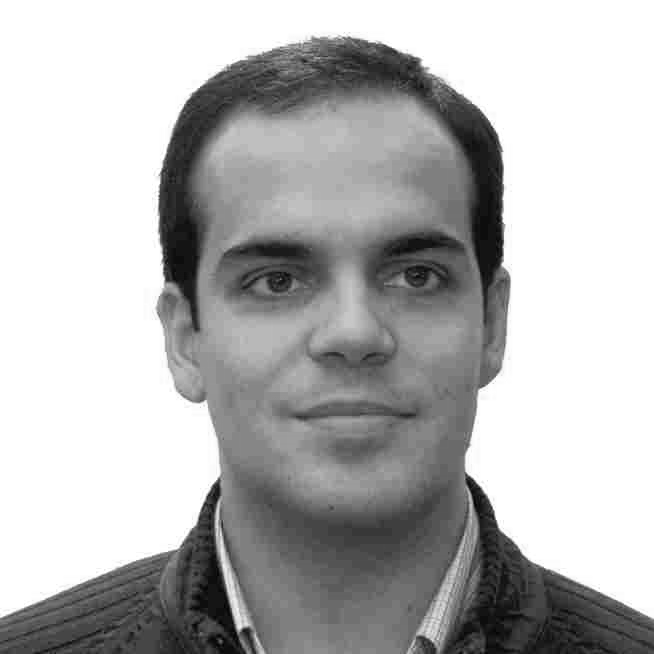
\includegraphics[width=\textwidth]{Camposinhos.jpg}
\end{subfigure}
\begin{subfigure}{.2\textwidth}
  \centering
  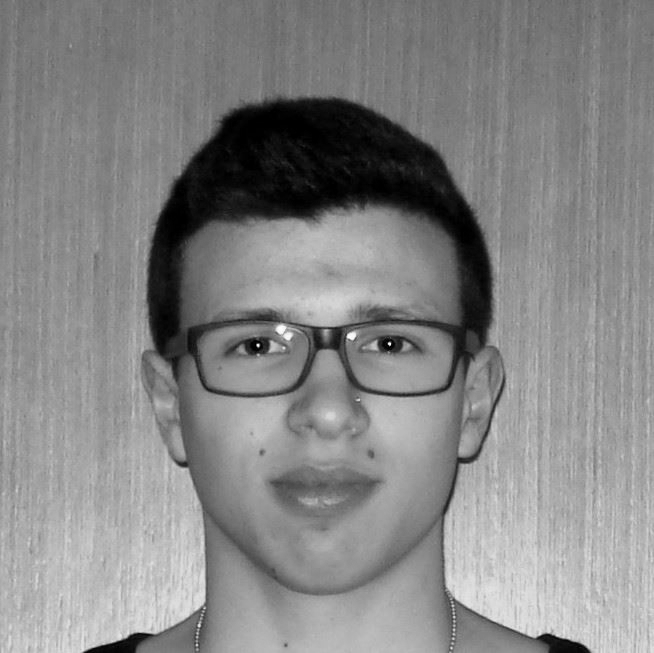
\includegraphics[width=\textwidth]{Oliveira.jpg}
\end{subfigure}
\begin{subfigure}{.2\textwidth}
  \centering
  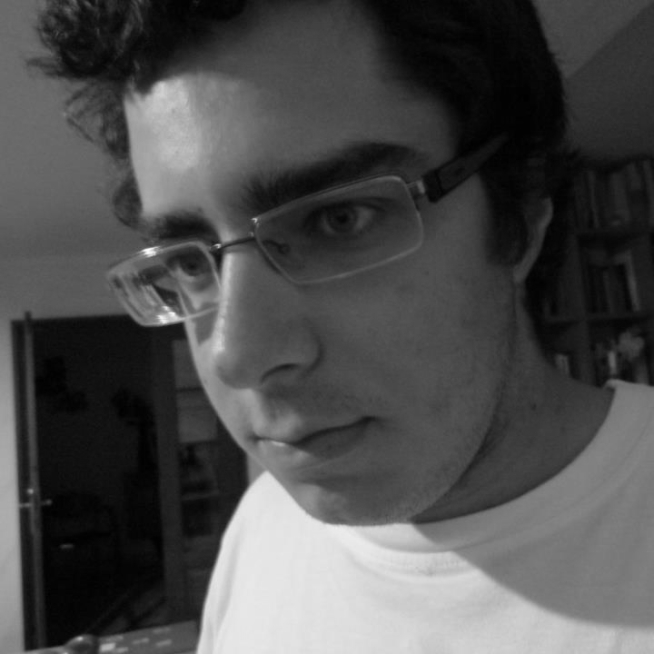
\includegraphics[width=\textwidth]{Santos.jpg}
\end{subfigure}
\end{figure}

\vspace{2cm}
Braga, 1 de junho de 2014

\end{center}

\end{titlepage}
%----------------------------------------------------------------------
\newpage
\phantom{placeholder} % doesn't appear on page
\thispagestyle{empty} % if want no header/footer
%----------------------------------------------------------------------
\tableofcontents
\phantom{placeholder} % doesn't appear on page
\thispagestyle{empty} % if want no header/footer
%----------------------------------------------------------------------
\newpage
\phantom{placeholder} % doesn't appear on page
\thispagestyle{empty} % if want no header/footer
%----------------------------------------------------------------------
\pagestyle{fancy}
\setlength{\headheight}{15.2pt}
\fancyhf{} % apagar as configurações actuais
\fancyfoot[LE,RO]{\thepage}
\fancyhead[LE,RO]{POO --- FitnessUM --- Grupo 14}
\setcounter{page}{0}
%----------------------------------------------------------------------

\chapter{Introdução}
\label{cap:intro}
O presente projecto enquadra-se na unidade curricular de Programação Orientada a Objectos do curso de Licenciatura em Engenharia 
Informática da Universidade do Minho.
O projecto pretende implementar uma aplicação, designada \emph{FitnessUM}, para registar e simular actividades desportivas de fitness.
A aplicação pretende foi desenvolvida em \emph{java} e pretende simular um ambiente de rede social.

\section{Objectivos}
\label{sec:obj}
(...)

De acordo com o enunciado \cite{enunciado}, os principais objectivos definidos para a aplicação são os seguintes (\emph{requisitos}):
\begin{itemize}
\item \textbf{req1:} (...);
\item \textbf{req2:} (...); 
\item (...); 
\end{itemize}

\section{Organização do Relatório}
\label{sec:org}
(...)

\chapter{Arquitectura e Descrição da Aplicação}
\label{cap:arq}
\section{Packages}
\label{sec:packages}
(...)
Model–view–controller (MVC) figura \ref{fig:mvc}.
(...)
\begin{figure}
\centering
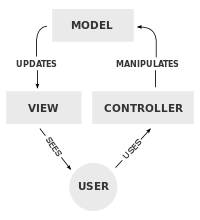
\includegraphics[width=4cm]{MVC-Process.png}
\caption{Diagrama com a relação típica dos componentes do MVC (ref.:\url{http://en.wikipedia.org/wiki/Model-view-controller}).}
\label{fig:mvc}
\end{figure}
(...)

De forma a manter uma estrutura de pastas partilhada entre os autores e um controlo de versões eficaz, 
foi utilizada a ferramenta open source \emph{GIT} (\url{http://git-scm.com/}), 
com repositório privado no bitbucket (\url{https://bitbucket.org/ruiOliveiras94/fitnessum-poo}).

falar também do Manager, Dataset, ...

\section{Descrição das Classes Principais}
\label{sec:classes}
(...)
A figura (...) apresenta o grafo de dependências dos vários ficheiros de código, obtido através do \emph{BlueJ}.

\chapter{Estruturas de Dados Principais}
\label{cap:estruturas}
(...)
\section{Class User}
\label{sec:user}
(...)
\section{Class Activity}
\label{sec:activity}
(...)
\section{Class Event}
\label{sec:event}
(...)

\chapter{Cálculo do Consumo de Calorias por Actividade}
\label{cap:calorias}
O procedimento de cálculo utilizado para estimar a quantidade de calorias dispendidas por actividade seguiu uma filosofia semelhante à utilizada 
na rede social \emph{Endomondo} (\url{www.endomondo.com}). 
Na figura \ref{fig:caloriasProcedimento} apresenta-se um diagrama explicativo do mesmo, onde se evidenciam duas vias: uma baseada na frequência 
cardíaca e outra no tipo de actividade.

Os dados básicos necessários para o cálculo das calorias dispendidas estão relacionados com o individuo e são:
\begin{itemize}
 \item Género;
 \item Características físicas --- peso, altura;
 \item Idade;
 \item Frequência cardíaca em repouso (no caso da via de cálculo baseada na frequência cardíaca).
\end{itemize}

Os dados complementares são:
\begin{itemize}
 \item Duração da actividade;
 \item O tipo de actividade (no caso da via de cálculo baseada no tipo de actividade);
 \item Frequência cardíaca média durante a actividade (no caso da via de cálculo baseada na frequência cardíaca).
\end{itemize}

\begin{figure}
\centering
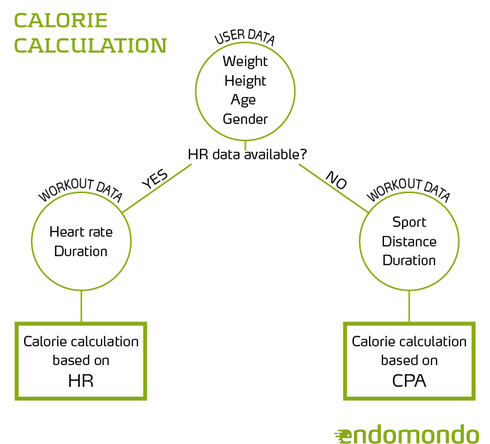
\includegraphics[width=7cm]{endomondoCalories.jpg}
\caption{Diagrama com o procedimento de cálculo adoptado para a estimativa do consumo de calorias por actividade (ref. \cite{endomondo}).}
\label{fig:caloriasProcedimento}
\end{figure}

\section{Cálculo Baseado na Frequência Cardíaca}
\label{sec:caloriasFcardio}
As formulações expostas na presente secção tiveram por base a aplicação web ``Heart Rate Based Calorie Burn Calculator'', 
da página \url{http://www.shapesense.com/fitness-exercise/calculators/}. Por uma questão de completitude apresentam-se todas as referências originais.
No cálculo pela via da frequência cardíaca um dos parâmetros fundamentais é o $VO2_{max}$, que é a capacidade máxima do corpo de um 
indivíduo em transportar e fazer uso de oxigênio durante um exercício físico incremental.
Este parâmetro pode ser estimado de acordo com \cite{VO2max}, com base na frequência cardíaca máxima ($MHR$) e em 
repouso ($RHR$) --- equação \ref{eq:VO2max}.
A frequência cardíaca máxima pode ser estimada com base na idade de acordo com \cite{MHR} --- equação \ref{eq:MHR}.
As calorias brutas dispendidas ($GCB$) foram estimadas de acordo com \cite{GCB} --- equação \ref{eq:GCB}.
Por fim, para se determinar o número de calorias efectivas ($NCB$) calculou-se a taxa metabólica basal ($BMR$) e a taxa de actividade ($RMRCB$)
A estimativa das calorias efectivas foi realizada de acordo com \cite{NCB} --- equações \ref{eq:NCB}, \ref{eq:RMRCB} e \ref{eq:BMR}.

\begin{equation} \label{eq:MHR} 
MHR = 208 - 0.7 \times Idade \text{\hspace*{0.3cm}[1/min]}
\end{equation}

\begin{equation} \label{eq:VO2max} 
VO2_{max} = 15.3 \times \frac{MHR}{RMR} \text{\hspace*{0.3cm}[ml/(kg.min)]}
\end{equation}

\begin{eqnarray} \label{eq:GCB}
\text{Homens:}&&\\ 
GCB &=& \frac{-55.0969 + 0.6309 \times HR + 0.1988 \times W + 0.2017 \times A}{4.184} \times 60 \times T \text{\hspace*{0.3cm}[kcal]}\nonumber\\
\text{Mulheres:}&&\nonumber\\ 
GCB &=& \frac{-20.4022 + 0.4472 \times HR + 0.1263 \times W + 0.074 \times A}{4.184} \times 60 \times T \text{\hspace*{0.3cm}[kcal]}\nonumber\\
\text{onde:}&& \nonumber\\
HR &=& \text{frequência cardíaca [1/min]}\nonumber\\ 
W &=& \text{Peso [kg]}\nonumber\\
A &=& \text{Idade [anos]}\nonumber\\
T &=& \text{Duração exercício [h]}\nonumber
\end{eqnarray}

\begin{equation} \label{eq:NCB} 
NCB = GCB - RMRCB \text{\hspace*{0.3cm}[kcal]}
\end{equation}

\begin{equation} \label{eq:RMRCB} 
RMRCB = \frac{BMR \times 1.1}{24} \times T \text{\hspace*{0.3cm}[kcal]}
\end{equation}

\begin{eqnarray} \label{eq:BMR}
\text{Homens:}&&\\
BMR &=& (13.75 \times W) + (5 \times H) - (6.76 \times A) + 66 \text{\hspace*{0.3cm}[kcal/24h]}\nonumber\\
\text{Mulheres:}&&\nonumber\\ 
BMR &=& (9.56 \times W) + (1.85 \times H) - 4.68 \times A) + 655 \text{\hspace*{0.3cm}[kcal/24h]}\nonumber\\
\text{onde:}&& \nonumber\\
H &=& \text{altura [cm]}\nonumber\\ 
&&\text{restantes referências na eq. \ref{eq:GCB}}\nonumber
\end{eqnarray}

\section{Cálculo Baseado no Tipo de Actividade}
\label{sec:caloriasMet}
Na ausência de dados relativos à frequência cardíaca do individuo, o cálculo do número de calorias dispendidas ($CB$) é efectuado com base 
no índice MET (``The Metabolic Equivalent of Task''). Este índice é uma medida fisiológica do custo energético de um dado exercício físico.
Com base nesta abordagem mais simplificada, as calorias dispendidas podem ser calculadas de acordo com a equação \ref{eq:CBmet}.

\begin{equation} \label{eq:CBmet} 
CB = MET \times W \times T \text{\hspace*{0.3cm}[kcal]}
\end{equation}

Os índices MET foram definidos de acordo com o ``Compendium of physical activities'' \cite{compendium}, da autoria do ``Healthy Lifestyles Research Center``, 
''School of Nutrition and Health Promotion`` da Arizona State University \url{https://sites.google.com/site/compendiumofphysicalactivities/}.
Na tabela \ref{tab:met} apresentam-se alguns valores típicos dos índices MET. 
De forma a adaptar os valores dos índices MET a cada índividuo (peso, altura e idade), foram aplicadas correcções de acordo com \cite{NCB} --- 
valor corrigido $CMET$ (eq. \ref{eq:CMET}), para mais detalhes ver \url{https://sites.google.com/site/compendiumofphysicalactivities/corrected-mets}.

\begin{table}
\caption {Valores típicos do índice MET (ref. \url{http://www.my-calorie-counter.com/mets_calculation.asp})} 
\label{tab:met}
\begin{center}
  \begin{tabular}{| c | l |}
    \hline                       
    METS & Activity\\
    \hline  
    \hline  
    1 & sitting quietly and watching television \\
    \hline  
    2 & walking, less than 2.0 mph, level ground, strolling, very slow \\
    \hline  
    3 & loading /unloading a car\\
    \hline  
    4 & bicycling, < 10 mph, leisure, to work or for pleasure\\
    \hline  
    (...) & (...)\\
    \hline  
    11 & running, 6.7 mph\\
    \hline  
    12 & fire fighter, general\\
    \hline  
  \end{tabular}
\end{center}
\end{table}

\begin{equation} \label{eq:CMET} 
CMET = MET \times \frac{3.5 \text{ ml/kg/min}}{RMRCB [\text{ ml/kg/min}]}
\end{equation}

\chapter{Cálculo da Forma dos Utilizadores}
\label{cap:forma}
A forma é um valor de 0 a 1. (Pode ser mudado alterando as variáveis \verb!MAX_FORMA! e \verb!MIN_FORMA!).

O cálculo da forma assume um número de dias nos quais todas as actividades feitas nesse intervalo têm influência para a forma 
(variável \verb!DIAS_RELEVANTES!). Se \verb!DIAS_RELEVANTES=24!, significa eu só as actividades nos últimos 24 dias têm influência para a forma.  
Isto serve para simular o facto de só as actividades mais recentes deverem ter influência na forma actual e quanto mais recentes as 
actividades, maior a influência na forma.

A cada dia é atribuído um ''peso``, o quanto esse dia vai valer para o cálculo final da forma. 
No entanto, não é feita uma distribuição equitativa dos pesos pelos dias. Dias mais distantes no tempo têm menos influência e portanto, 
menos peso. Essa “menos influência” é dada por uma taxa (variável TAXA) que representa o decréscimo na forma resultante de ficar 1 dia sem 
fazer nenhuma actividade. Se \verb!TAXA=0.05!, significa que cada dia que se ande para trás, tem -5\% de influência no cálculo da forma.
A contribuição para a forma de cada dia é calculado multiplicando o peso desse dia pelo quociente entre o número de minutos que o utilizador 
fez de uma actividade e o nº de minutos recomendado para essa actividade (nº de minutos recomendado para 1 actividade = Intensidade). 
Somadas todas as contribuições de cada dia, tem-se a forma final.

\chapter{Simulação de Eventos}
\label{cap:simula}
(...)

\chapter{Conclusões}
\label{cap:concl}
(...)

\bibliographystyle{plain}
\bibliography{relatorio-POO-CamposinhosOliveiraSantos}

\appendix
\chapter{Documentação do Código}
\label{anex:doc}

\chapter{Demo da aplicação}
\label{anex:demo}




\end{document}
